\section{A Brief Survey of Automated Machine Learning}\label{sec:dttts.survey}

We provide a full-stack pipeline for a machine learning procedure as displayed in Fig.~\ref{fig:automl} and a general taxonomy on different components of AutoML~\citep{hutter2019automl,zoller2019automl,he2019automl}. We pay particular attention to hyper-parameter optimization, neural architecture search and meta learning later in separate subsections. The following structure is partly inspired by various surveys mentioned in the references.

\begin{figure}[ht]
    \centering
    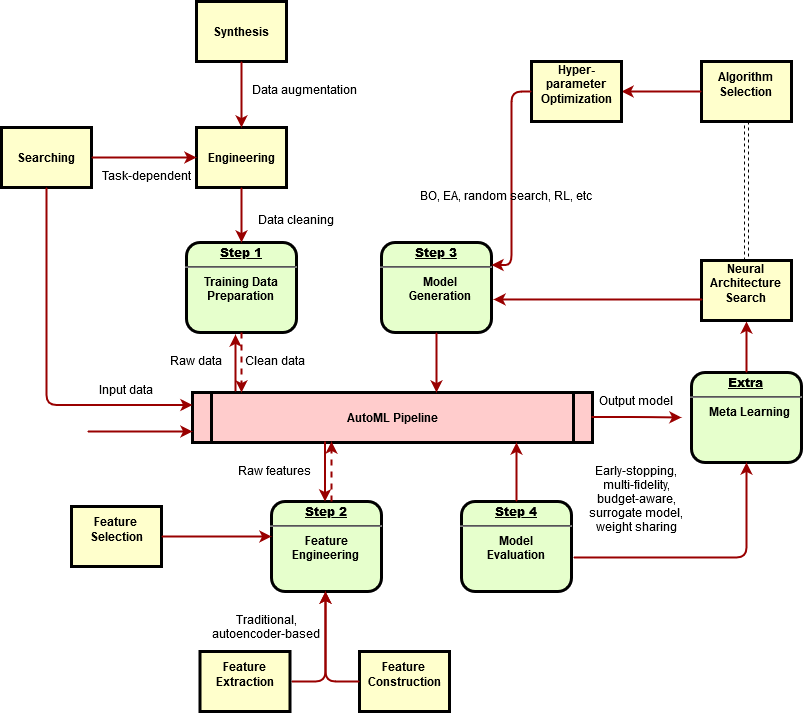
\includegraphics[width=\textwidth]{Chapter6/img/automl.png}
    \caption{The full-stack pipeline of a machine learning task.}
    \label{fig:automl}
\end{figure}


\subsection{The AutoML taxonomy}\label{sec:dttts.survey.taxonomy}

\paragraph{Data preparation}

\begin{itemize}
    \item Data collection
    \begin{itemize}
        \item Web searching, however data could be ill-labeled or inaccurate, semi-supervised or self-labeling methods are required;
        \item Data synthesis when not enough data available, mainly using data augmentation.
    \end{itemize}
    \item Data cleaning
    \begin{itemize}
        \item Standardization;
        \item Scaling;
	    \item Binarization of numerical (discrete or continuous) attributes;
	    \item One-hot encoding for categorical attributes;
	    \item Imputation (e.g. with mean values).
    \end{itemize}
    \item Feature engineering
\end{itemize}

\paragraph{Feature engineering}

\begin{itemize}
    \item Feature selection
    \begin{itemize}
        \item Subset generation, using some (random) search strategy (simulated annealing, genetic algorithms);
        \item Subset evaluation with filter methods, wrapper methods or embedded methods (deep learning, decision trees, etc);
        \item Subset validation.
    \end{itemize}
    \item Feature extraction (alters the features)
    \begin{itemize}
        \item Dimensionality reduction techniques like PCA, ICA, LDA, etc;
        \item Autoencoder-based methods.
    \end{itemize}
    \item Feature construction
    \begin{itemize}
        \item Searching methods such as tree-based approaches, genetic algorithms;
        \item Annotation-based approaches.
    \end{itemize}
\end{itemize}

\paragraph{Pipeline generation} 
This is the most important part to be further detailed.

\begin{itemize}
    \item FMS (full model selection) or CASH (combined algorithm and hyper-parameter optimization)
    \begin{itemize}
        \item Model/Algorithm selection;
        \item HPO (hyper-parameter optimization).
    \end{itemize}
    \item NAS (neural architecture search)
    \item Ensembling, since choosing one single full model maybe a waste
    \item Metal learning
\end{itemize}

\paragraph{Model evaluation or estimation}

\begin{itemize}
    \item Complete training (time and resource-consuming especially)
    \item Multi-fidelity (low resolution, subset of data, not only for DL)
    \item Early-stopping (mostly for DL)
    \item Surrogate model (not only for DL)
    \item Weight sharing (DL-specific)
    \item Resource/budget-aware (computational cost is added to the loss)
\end{itemize}
    
    
\paragraph{Existing (open source) AutoML frameworks} 
TPOT, AutoKeras, auto-sklearn, Transmogrif, MLBox

\subsection{Hyper-parameter optimization}\label{sec:dttts.survey.hpo}

\paragraph{Black-box optimization}

\begin{itemize}
    \item Model-free
    \begin{itemize}
        \item \Random, \Grid;
        \item Population-based as \CMAES, more precisely genetic algorithms, evolutionary algorithms, evolutionary strategies, and particle swarm optimization: maintain a population, then improve this population by applying mutations or crossovers.
    \end{itemize}
    \item Model-based (in particular Bayesian optimization)
    \begin{itemize}
        \item Traditional Bayesian optimization with various surrogate models and acquisition functions, like \GPUCB, \PI, \EI with Gaussian processes and \SMAC with random forests; 
        \item Atypical Bayesian optimization \TPE;
        \item Thompson sampling-based \DTTTS.
    \end{itemize}
\end{itemize}

\paragraph{Gray-box optimization}

\begin{itemize}
    \item Multi-fidelity Optimization
    \begin{itemize}
        \item Bandit-based algorithm \Hyperband, that introduces the concept of partial training;
        \item `Auto-WEKA` appears to be the only paper that uses only one or a few of the cross-validation folds;
        \item Bayesian optimization + partial training = \BOHB;
        \item Learning curve.
    \end{itemize}
    \item Gradient-based
\end{itemize}

% - Current Benchmark (they are mostly designed for a continuous search space)
%     - `Random Search`
%     - `CMA-ES`
%     - `SMAC`
%     - `TPE`
%     - `Hyperband`
%     - `BOHB`

\subsection{Meta learning}\label{sec:dttts.survey.meta}

\subsection{Neural architecture search}\label{sec:dttts.survey.nas}

\paragraph{Model generation}

\begin{itemize}
    \item Elemental operations
    \begin{itemize}
        \item Convolution;
        \item Pooling (max-pooling, average-pooling, attention);
        \item Concatenation;
        \item Addition;
        \item Skip connection (ResNet).
    \end{itemize}
    \item Model structures
    \begin{itemize}
        \item Entire structure;
        \item Cell-based structure (normal cell or reduction cell like `NASNet`): internal cell design with human-designed operations;
        \item Progressive structure;
        \item Morphism-based structure.
    \end{itemize}
\end{itemize}

\paragraph{Hyper-parameter Optimization}

\begin{itemize}
    \item Classical HPO methods
    \item RL-based methods
\end{itemize}
